
%%--------------------------------------------------
%% Serway: Physics for Scientists and Engineers
%%--------------------------------------------------


%% Chapter 04: Motion in Two Dimensions
%%--------------------------------------------------


%% Table of Contents
%%--------------------------------------------------

%% 4.1 The Position, Velocity, and Acceleration Vectors
%% 4.2 Two-Dimensional Motion with Constant Acceleration
%% 4.4 Projectile Motion
%% 4.5 The Particle in Uniform Circular Motion
%% 4.6 Tangential and Radial Acceleration
%% 4.7 Relative Velocity and Relative Acceleration


%% Serway Multiple Choice Questions
%%--------------------------------------------------
\element{serway-mc}{
\begin{question}{serway-ch04-q01}
    At $t = 0$, a particle leaves the origin with a velocity of \SI{9.0}{\meter\per\second} in the positive $y$ direction and moves in the $xy$ plane with a constant acceleration of
        $\left( 2.0\hat{\imath} - 4.0\hat{\jmath} \right)\,\si{\meter\per\second\squared}$.
    At the instant the $x$ coordinate of the particle is \SI{15}{\meter},
        what is the speed of the particle?
    \begin{multicols}{3}
    \begin{choices}
      \correctchoice{\SI{10}{\meter\per\second}}
        \wrongchoice{\SI{16}{\meter\per\second}}
        \wrongchoice{\SI{12}{\meter\per\second}}
        \wrongchoice{\SI{14}{\meter\per\second}}
        \wrongchoice{\SI{26}{\meter\per\second}}
    \end{choices}
    \end{multicols}
\end{question}
}

\element{serway-mc}{
\begin{question}{serway-ch04-q02}
    A particle starts from the origin at $t = 0$ with a velocity of $6.0\hat{\imath}\,\si{\meter\per\second}$ and moves in the $xy$ plane with a constant acceleration of
        $\left( -2.0\hat{\imath} + 4.0\hat{\jmath} \right)\,\si{\meter\per\second\squared}$.
    At the instant the particle achieves its maximum positive $x$ coordinate,
        how far is it from the origin?
    \begin{multicols}{3}
    \begin{choices}
        \wrongchoice{\SI{36}{\meter}}
      \correctchoice{\SI{20}{\meter}}
        \wrongchoice{\SI{45}{\meter}}
        \wrongchoice{\SI{27}{\meter}}
        \wrongchoice{\SI{37}{\meter}}
    \end{choices}
    \end{multicols}
\end{question}
}

\element{serway-mc}{
\begin{question}{serway-ch04-q03}
    A particle leaves the origin with a velocity of \SI{7.2}{\meter\per\second} in the positive $y$ direction and moves in the $xy$ plane with a constant acceleration of
        $\left( 3.0\hat{\imath} - 2.0\hat{\jmath} \right)\,\si{\meter\per\second\squared}$.
    At the instant the particle moves back across the $x$ axis ($y = 0$),
        what is the value of its $x$ coordinate?
    \begin{multicols}{3}
    \begin{choices}
        \wrongchoice{\SI{65}{\meter}}
        \wrongchoice{\SI{91}{\meter}}
        \wrongchoice{\SI{54}{\meter}}
      \correctchoice{\SI{78}{\meter}}
        \wrongchoice{\SI{86}{\meter}}
    \end{choices}
    \end{multicols}
\end{question}
}

\element{serway-mc}{
\begin{question}{serway-ch04-q04}
    At $t = 0$, a particle leaves the origin with a velocity of \SI{5.0}{\meter\per\second} in the positive $y$ direction.
    Its acceleration is given by
        $\vec{\mathbf{a}} = \left( 3.0\hat{\imath} - 2.0\hat{\jmath} \right)\,\si{\meter\per\second\squared}$.
    At the instant the particle reaches its maximum $y$ coordinate how far is the particle from the origin?
    \begin{multicols}{3}
    \begin{choices}
      \correctchoice{\SI{11}{\meter}}
        \wrongchoice{\SI{16}{\meter}}
        \wrongchoice{\SI{22}{\meter}}
        \wrongchoice{\SI{29}{\meter}}
        \wrongchoice{\SI{19}{\meter}}
    \end{choices}
    \end{multicols}
\end{question}
}

\element{serway-mc}{
\begin{question}{serway-ch04-q05}
    A particle moves in the $xy$ plane with a constant acceleration given by
        $\vec{\mathbf{a}} = -4.0\hat{\jmath}\,\si{\meter\per\second\squared}$.
    At $t = 0$, its position and velocity are
        $10\hat{\imath}\,\si{\meter}$ and
        $\left( -2.0\hat{\imath} + 8.0\hat{\jmath} \right)\,\si{\meter\per\second}$,
        respectively.
    What is the distance from the origin to the particle at $t = \SI{2.0}{\second}$?
    \begin{multicols}{3}
    \begin{choices}
        \wrongchoice{\SI{6.4}{\meter}}
      \correctchoice{\SI{10}{\meter}}
        \wrongchoice{\SI{8.9}{\meter}}
        \wrongchoice{\SI{2.0}{\meter}}
        \wrongchoice{\SI{6.2}{\meter}}
    \end{choices}
    \end{multicols}
\end{question}
}

\element{serway-mc}{
\begin{question}{serway-ch04-q06}
    A particle starts from the origin at $t = 0$ with a velocity of
        $\left( 16\hat{\imath} - 12\hat{\jmath} \right)\,\si{\meter\per\second}$
        and moves in the $xy$ plane with a constant acceleration of
        $\vec{\mathbf{a}} = \left( 3.0\hat{\imath} - 6.0\hat{\jmath}\right)\,\si{\meter\per\second\squared}$.
    What is the speed of the particle at $t = \SI{2.0}{\second}$?
    \begin{multicols}{3}
    \begin{choices}
        \wrongchoice{\SI{52}{\meter\per\second}}
        \wrongchoice{\SI{39}{\meter\per\second}}
        \wrongchoice{\SI{46}{\meter\per\second}}
      \correctchoice{\SI{33}{\meter\per\second}}
        \wrongchoice{\SI{43}{\meter\per\second}}
    \end{choices}
    \end{multicols}
\end{question}
}

\element{serway-mc}{
\begin{question}{serway-ch04-q07}
    At $t = 0$, a particle leaves the origin with a velocity of \SI{12}{\meter\per\second} in the positive $x$ direction and moves in the $xy$ plane with a constant acceleration of
        $\left( -2.0\hat{\imath} + 4.0\hat{\jmath} \right)\,\si{\meter\per\second}$.
    At the instant the $y$ coordinate of the particle is \SI{18}{\meter},
        what is the $x$ coordinate of the particle?
    \begin{multicols}{3}
    \begin{choices}
        \wrongchoice{\SI{30}{\meter}}
        \wrongchoice{\SI{21}{\meter}}
      \correctchoice{\SI{27}{\meter}}
        \wrongchoice{\SI{24}{\meter}}
        \wrongchoice{\SI{45}{\meter}}
    \end{choices}
    \end{multicols}
\end{question}
}

\element{serway-mc}{
\begin{question}{serway-ch04-q08}
    The initial speed of a cannon ball is \SI{0.20}{\kilo\meter\per\second}.
    If the ball is to strike a target that is at a horizontal distance of \SI{3.0}{\kilo\meter} from the cannon,
        what is the minimum time of flight for the ball?
    \begin{multicols}{3}
    \begin{choices}
      \correctchoice{\SI{16}{\second}}
        \wrongchoice{\SI{21}{\second}}
        \wrongchoice{\SI{24}{\second}}
        \wrongchoice{\SI{14}{\second}}
        \wrongchoice{\SI{19}{\second}}
    \end{choices}
    \end{multicols}
\end{question}
}

\element{serway-mc}{
\begin{question}{serway-ch04-q09}
    A ball is thrown horizontally from the top of a building \SI{0.10}{\kilo\meter} high.
    The ball strikes the ground at a point \SI{65}{\meter} horizontally away from and below the point of release.
    What is the speed of the ball just before it strikes the ground?
    \begin{multicols}{3}
    \begin{choices}
        \wrongchoice{\SI{43}{\meter\per\second}}
      \correctchoice{\SI{47}{\meter\per\second}}
        \wrongchoice{\SI{39}{\meter\per\second}}
        \wrongchoice{\SI{36}{\meter\per\second}}
        \wrongchoice{\SI{14}{\meter\per\second}}
    \end{choices}
    \end{multicols}
\end{question}
}

\element{serway-mc}{
\begin{question}{serway-ch04-q10}
    A baseball is hit at ground level.
    The ball is observed to reach its maximum height above ground level \SI{3.0}{\second} after being hit.
    And \SI{2.5}{\second} after reaching this maximum height,
        the ball is observed to barely clear a fence that is \SI{97.5}{\meter} from where it was hit.
    How high is the fence?
    \begin{multicols}{3}
    \begin{choices}
        \wrongchoice{\SI{8.2}{\meter}}
        \wrongchoice{\SI{15.8}{\meter}}
      \correctchoice{\SI{13.4}{\meter}}
        \wrongchoice{\SI{11.0}{\meter}}
        \wrongchoice{\SI{4.9}{\meter}}
    \end{choices}
    \end{multicols}
\end{question}
}

\element{serway-mc}{
\begin{question}{serway-ch04-q11}
    A rock is projected from the edge of the top of a building with an initial velocity of \SI{12.2}{\meter\per\second} at an angle of \ang{53} above the horizontal.
    The rock strikes the ground a horizontal distance of \SI{25}{\meter} from the base of the building.
    Assume that the ground is level and that the side of the building is vertical.
    How tall is the building?
    \begin{multicols}{3}
    \begin{choices}
        \wrongchoice{\SI{25.3}{\meter}}
        \wrongchoice{\SI{29.6}{\meter}}
        \wrongchoice{\SI{27.4}{\meter}}
      \correctchoice{\SI{23.6}{\meter}}
        \wrongchoice{\SI{18.9}{\meter}}
    \end{choices}
    \end{multicols}
\end{question}
}

\element{serway-mc}{
\begin{question}{serway-ch04-q12}
    A projectile is thrown from the top of a building with an initial velocity of \SI{30}{\meter\per\second} in the horizontal direction.
    If the top of the building is \SI{30}{\meter} above the ground,
        how fast will the projectile be moving just before it strikes the ground?
    \begin{multicols}{3}
    \begin{choices}
        \wrongchoice{\SI{35}{\meter\per\second}}
      \correctchoice{\SI{39}{\meter\per\second}}
        \wrongchoice{\SI{31}{\meter\per\second}}
        \wrongchoice{\SI{43}{\meter\per\second}}
        \wrongchoice{\SI{54}{\meter\per\second}}
    \end{choices}
    \end{multicols}
\end{question}
}

\element{serway-mc}{
\begin{question}{serway-ch04-q13}
    A rifle is aimed horizontally at the center of a large target \SI{60}{\meter} away.
    The initial speed of the bullet is \SI{240}{\meter\per\second}.
    What is the distance from the center of the target to the point where the bullet strikes the target?
    \begin{multicols}{3}
    \begin{choices}
        \wrongchoice{\SI{48}{\centi\meter}}
        \wrongchoice{\SI{17}{\centi\meter}}
      \correctchoice{\SI{31}{\centi\meter}}
        \wrongchoice{\SI{69}{\centi\meter}}
        \wrongchoice{\SI{52}{\centi\meter}}
    \end{choices}
    \end{multicols}
\end{question}
}

\element{serway-mc}{
\begin{question}{serway-ch04-q14}
    A rock is thrown from the edge of the top of a \SI{100}{\foot} tall building at some unknown angle above the horizontal.
    The rock strikes the ground a horizontal distance of \SI{160}{\foot} from the base of the building \SI{5.0}{\second} after being thrown.
    Assume that the ground is level and that the side of the building is vertical.
    Determine the speed with which the rock was thrown.
    \begin{multicols}{3}
    \begin{choices}
        \wrongchoice{\SI{72}{\foot\per\second}}
        \wrongchoice{\SI{77}{\foot\per\second}}
      \correctchoice{\SI{68}{\foot\per\second}}
        \wrongchoice{\SI{82}{\foot\per\second}}
        \wrongchoice{\SI{87}{\foot\per\second}}
    \end{choices}
    \end{multicols}
\end{question}
}

\element{serway-mc}{
\begin{question}{serway-ch04-q15}
    An airplane flies horizontally with a speed of \SI{300}{\meter\per\second} at an altitude of \SI{400}{\meter}.
    Assume that the ground is level.
    At what horizontal distance from a target must the pilot release a bomb so as to hit the target?
    \begin{multicols}{3}
    \begin{choices}
        \wrongchoice{\SI{3.0}{\kilo\meter}}
        \wrongchoice{\SI{2.4}{\kilo\meter}}
        \wrongchoice{\SI{3.3}{\kilo\meter}}
      \correctchoice{\SI{2.7}{\kilo\meter}}
        \wrongchoice{\SI{1.7}{\kilo\meter}}
    \end{choices}
    \end{multicols}
\end{question}
}

\element{serway-mc}{
\begin{question}{serway-ch04-q16}
    An object moving at a constant speed requires \SI{6.0}{\second} to go once around a circle with a diameter of \SI{4.0}{\meter}.
    What is the magnitude of the instantaneous acceleration of the particle during this time?
    \begin{multicols}{3}
    \begin{choices}
      \correctchoice{\SI{2.2}{\meter\per\second\squared}}
        \wrongchoice{\SI{2.7}{\meter\per\second\squared}}
        \wrongchoice{\SI{3.3}{\meter\per\second\squared}}
        \wrongchoice{\SI{3.8}{\meter\per\second\squared}}
        \wrongchoice{\SI{4.4}{\meter\per\second\squared}}
    \end{choices}
    \end{multicols}
\end{question}
}

\element{serway-mc}{
\begin{question}{serway-ch04-q17}
    A particle moves at a constant speed in a circular path with a radius of \SI{2.06}{\centi\meter}.
    If the particle makes four revolutions each second,
        what is the magnitude of its acceleration?
    \begin{multicols}{3}
    \begin{choices}
        \wrongchoice{\SI{20}{\meter\per\second\squared}}
        \wrongchoice{\SI{18}{\meter\per\second\squared}}
      \correctchoice{\SI{13}{\meter\per\second\squared}}
        \wrongchoice{\SI{15}{\meter\per\second\squared}}
        \wrongchoice{\SI{24}{\meter\per\second\squared}}
    \end{choices}
    \end{multicols}
\end{question}
}

\element{serway-mc}{
\begin{question}{serway-ch04-q18}
    A race car moving with a constant speed of \SI{60}{\meter\per\second} completes one lap around a circular track in \SI{50}{\second}.
    What is the magnitude of the acceleration of the race car?
    \begin{multicols}{3}
    \begin{choices}
        \wrongchoice{\SI{8.8}{\meter\per\second\squared}}
      \correctchoice{\SI{7.5}{\meter\per\second\squared}}
        \wrongchoice{\SI{9.4}{\meter\per\second\squared}}
        \wrongchoice{\SI{6.3}{\meter\per\second\squared}}
        \wrongchoice{\SI{5.3}{\meter\per\second\squared}}
    \end{choices}
    \end{multicols}
\end{question}
}

\element{serway-mc}{
\begin{question}{serway-ch04-q19}
    At the lowest point in a vertical dive (radius = \SI{0.58}{\kilo\meter}),
        an airplane has a speed of \SI{300}{\kilo\meter\per\hour} which is not changing.
    Determine the magnitude of the acceleration of the pilot at this lowest point.
    \begin{multicols}{3}
    \begin{choices}
        \wrongchoice{\SI{26}{\meter\per\second\squared}}
        \wrongchoice{\SI{21}{\meter\per\second\squared}}
        \wrongchoice{\SI{16}{\meter\per\second\squared}}
      \correctchoice{\SI{12}{\meter\per\second\squared}}
        \wrongchoice{\SI{8.8}{\meter\per\second\squared}}
    \end{choices}
    \end{multicols}
\end{question}
}

\element{serway-mc}{
\begin{question}{serway-ch04-q20}
    A carnival Ferris wheel has a \SI{15}{\meter} radius and completes five turns about its horizontal axis every minute.
    What is the acceleration of a passenger at his lowest point during the ride?
    \begin{choices}
        \wrongchoice{\SI{5.7}{\meter\per\second\squared} downward}
      \correctchoice{\SI{4.1}{\meter\per\second\squared} upward}
        \wrongchoice{\SI{14}{\meter\per\second\squared} downward}
        \wrongchoice{\SI{4.1}{\meter\per\second\squared} downward}
        \wrongchoice{\SI{19}{\meter\per\second\squared} downward}
    \end{choices}
\end{question}
}

\element{serway-mc}{
\begin{question}{serway-ch04-q21}
    A space station of diameter \SI{80}{\meter} is turning about its axis at a constant rate.
    If the acceleration of the outer rim of the station is \SI{2.5}{\meter\per\second\squared},
        what is the period of revolution of the space station?
    \begin{multicols}{3}
    \begin{choices}
        \wrongchoice{\SI{22}{\second}}
        \wrongchoice{\SI{19}{\second}}
      \correctchoice{\SI{25}{\second}}
        \wrongchoice{\SI{28}{\second}}
        \wrongchoice{\SI{40}{\second}}
    \end{choices}
    \end{multicols}
\end{question}
}

\element{serway-mc}{
\begin{question}{serway-ch04-q22}
    A car travels counterclockwise around a flat circle of radius \SI{0.25}{\kilo\meter} at a constant speed of \SI{20}{\meter\per\second}.
    When the car is at point $A$ as shown in the figure,
    \begin{center}
    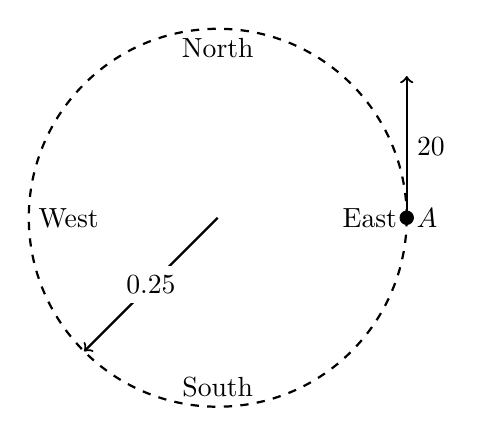
\begin{tikzpicture}[scale=1.2]
        %% Circle
        \draw[dashed,thick] (0,0) circle (2cm);
        \draw[thick,->] (0,0) -- ++(225:2) node[pos=0.5,anchor=center,fill=white] {\SI{0.25}{\kilo\meter}};
        %% Compass Labels
        \node[anchor=south] at (0,-2) {South};
        \node[anchor=north] at (0,+2) {North};
        \node[anchor=west] at (-2,0) {West};
        \node[anchor=east] at (+2,0) {East};
        %% Vectors
        \draw[fill] (2,0) circle (2pt) node[anchor=west] {$A$};
        \draw[thick,->] (2,0) -- ++(90:1.5cm)
            node[pos=0.5,anchor=west] {\SI{20}{\meter\per\second}};
    \end{tikzpicture}
    \end{center}
        what is the car’s acceleration?
    \begin{multicols}{2}
    \begin{choices}
        %% NOTE: A was duplicate of C
        %\wrongchoice{\SI{1.6}{\meter\per\second\squared}, east}
        %% NOTE: questionmult?  so dup is not significant?
        \wrongchoice{\SI{1.6}{\meter\per\second\squared}, south}
        \wrongchoice{Zero}
        \wrongchoice{\SI{1.6}{\meter\per\second\squared}, east}
        \wrongchoice{\SI{1.6}{\meter\per\second\squared}, north}
      \correctchoice{\SI{1.6}{\meter\per\second\squared}, west}
    \end{choices}
    \end{multicols}
\end{question}
}

\element{serway-mc}{
\begin{question}{serway-ch04-q23}
    A particle moves along a circular path having a radius of \SI{2.0}{\meter}.
    At an instant when the speed of the particle is equal to \SI{3.0}{\meter\per\second} and changing at the rate of \SI{5.0}{\meter\per\second\squared},
        what is the magnitude of the total acceleration of the particle?
    \begin{multicols}{3}
    \begin{choices}
        \wrongchoice{\SI{7.5}{\meter\per\second\squared}}
        \wrongchoice{\SI{6.0}{\meter\per\second\squared}}
        \wrongchoice{\SI{5.4}{\meter\per\second\squared}}
      \correctchoice{\SI{6.7}{\meter\per\second\squared}}
        \wrongchoice{\SI{4.5}{\meter\per\second\squared}}
    \end{choices}
    \end{multicols}
\end{question}
}

\element{serway-mc}{
\begin{question}{serway-ch04-q24}
    A car travels in a flat circle of radius $R$.
    At a certain instant the velocity of the car is \SI{20}{\meter\per\second} north,
        and the total acceleration of the car is \SI{2.5}{\meter\per\second\squared} \ang{37} south of west.
    Which of the following is correct?
    \begin{choices}
        \wrongchoice{$R = \SI{0.40}{\kilo\meter}$, and the car's speed is decreasing.}
      \correctchoice{$R = \SI{0.20}{\kilo\meter}$, and the car's speed is decreasing.}
        \wrongchoice{$R = \SI{0.20}{\kilo\meter}$, and the car's speed is increasing.}
        \wrongchoice{$R = \SI{0.16}{\kilo\meter}$, and the car's speed is increasing.}
        \wrongchoice{$R = \SI{0.16}{\kilo\meter}$, and the car's speed is decreasing.}
    \end{choices}
\end{question}
}

\element{serway-mc}{
\begin{question}{serway-ch04-q25}
    A car travels in a flat circle of radius $R$.
    At a certain instant the velocity of the car is \SI{24}{\meter\per\second} west,
    and the total acceleration of the car is \SI{2.5}{\meter\per\second\squared} \ang{53} north of west.
    Which of the following is correct?
    \begin{choices}
      \correctchoice{$R = \SI{0.29}{\kilo\meter}$, and the car's speed is increasing.}
        \wrongchoice{$R = \SI{0.23}{\kilo\meter}$, and the car's speed is decreasing.}
        \wrongchoice{$R = \SI{0.23}{\kilo\meter}$, and the car's speed is increasing.}
        \wrongchoice{$R = \SI{0.29}{\kilo\meter}$, and the car's speed is decreasing}
        \wrongchoice{$R = \SI{0.29}{\kilo\meter}$, and the car's speed is constant.}
    \end{choices}
\end{question}
}

\element{serway-mc}{
\begin{question}{serway-ch04-q26}
    A stunt pilot performs a circular dive of radius \SI{800}{\meter}.
    At the bottom of the dive (point $B$ in the figure)
    \begin{center}
    \begin{tikzpicture}
        %% Coordinates
        \draw[->] (-3,-3) -- ++(90:1) node[anchor=south] {$\hat{\jmath}$};
        \draw[->] (-3,-3) -- ++(0:1) node[anchor=west] {$\hat{\imath}$};
        %% Pendulum
        \draw[->] (0,0) -- (310:3)
            node[pos=0.5,anchor=center,fill=white] {\SI{800}{\meter}};
        \draw[dashed] (225:3) arc (225:330:3);
        \draw[fill] (0,-3) circle (2pt) node[anchor=north] {$B$};
        \draw[thick,->] (0,-3) -- ++ (0:2);
    \end{tikzpicture}
    \end{center}
        the pilot has a speed of \SI{200}{\meter\per\second} which at that instant is increasing at a rate of \SI{20}{\meter\per\second\squared}.
    What acceleration does the pilot have at point $B$?
    \begin{multicols}{2}
    \begin{choices}
        \wrongchoice{$\left(  50\hat{\imath} + 20\hat{\jmath} \right)\,\si{\meter\per\second\squared}$}
        \wrongchoice{$\left(  20\hat{\imath} - 50\hat{\jmath} \right)\,\si{\meter\per\second\squared}$}
      \correctchoice{$\left(  20\hat{\imath} + 50\hat{\jmath} \right)\,\si{\meter\per\second\squared}$}
        \wrongchoice{$\left( -20\hat{\imath} + 50\hat{\jmath} \right)\,\si{\meter\per\second\squared}$}
        \wrongchoice{$\left( -50\hat{\imath} + 20\hat{\jmath} \right)\,\si{\meter\per\second\squared}$}
        %% NOTE: add one for symmetry, gravity makes this a good one!!
        \wrongchoice{$\left(  20\hat{\imath} + 40\hat{\jmath} \right)\,\si{\meter\per\second\squared}$}
    \end{choices}
    \end{multicols}
\end{question}
}

\element{serway-mc}{
\begin{question}{serway-ch04-q27}
    The speed of a particle moving in a circle \SI{2.0}{\meter} in radius increases at the constant rate of \SI{4.4}{\meter\per\second\squared}.
    At an instant when the magnitude of the total acceleration is \SI{6.0}{\meter\per\second\squared},
        what is the speed of the particle?
    \begin{multicols}{3}
    \begin{choices}
        \wrongchoice{\SI{3.9}{\meter\per\second}}
      \correctchoice{\SI{2.9}{\meter\per\second}}
        \wrongchoice{\SI{3.5}{\meter\per\second}}
        \wrongchoice{\SI{3.0}{\meter\per\second}}
        \wrongchoice{\SI{1.4}{\meter\per\second}}
    \end{choices}
    \end{multicols}
\end{question}
}

\element{serway-mc}{
\begin{question}{serway-ch04-q28}
    A car travels in a flat circle of radius R.
    At a certain instant the velocity of the car is \SI{24}{\meter\per\second} west,
        and the acceleration of the car has components of \SI{2.4}{\meter\per\second\squared} east and \SI{1.8}{\meter\per\second\squared} south.
    What is the radius of the circle?
    \begin{multicols}{3}
    \begin{choices}
        \wrongchoice{\SI{0.24}{\kilo\meter}}
        \wrongchoice{\SI{0.19}{\kilo\meter}}
      \correctchoice{\SI{0.32}{\kilo\meter}}
        \wrongchoice{\SI{0.14}{\kilo\meter}}
        \wrongchoice{\SI{0.27}{\kilo\meter}}
    \end{choices}
    \end{multicols}
\end{question}
}

\element{serway-mc}{
\begin{question}{serway-ch04-q29}
    A particle moves in the $xy$ plane in a circle centered on the origin.
    At a certain instant the velocity and acceleration of the particle are
        $\left(6.0\hat{\imath}\right)\,\si{\meter\per\second}$ and
        $\left(3.0\hat{\imath} + 4.0\hat{\jmath}\right)\,\si{\meter\per\second\squared}$.
    What are the $x$ and $y$ coordinates of the particle at this moment?
    \begin{choices}
      \correctchoice{$x = \SI{0}{\meter}$, $y = \SI{-9.0}{\meter}$}
        \wrongchoice{$x = \SI{0}{\meter}$, $y = \SI{+7.2}{\meter}$}
        \wrongchoice{$x = \SI{0}{\meter}$, $y = \SI{+9.0}{\meter}$}
        \wrongchoice{$x = \SI{0}{\meter}$, $y = \SI{-7.2}{\meter}$}
        \wrongchoice{$x = \SI{6.0}{\meter}$, $y = \SI{-9.0}{\meter}$}
    \end{choices}
\end{question}
}

\element{serway-mc}{
\begin{question}{serway-ch04-q30}
    A particle moves in the $xy$ plane in a circle centered on the origin.
    At a certain instant the velocity and acceleration of the particle are
        \SI[parse-numbers=false]{4.0\hat{\jmath}}{\meter\per\second} and
        $\left( -3.0\hat{\imath} - 2.0\hat{\jmath} \right)\,\si{\meter\per\second\squared}$.
    What are the $x$ and $y$ coordinates of the particle at this moment?
    \begin{choices}
        \wrongchoice{$x = \SI{-4.4}{\meter}$, $y = \SI{0.0}{\meter}$}
      \correctchoice{$x = \SI{+5.3}{\meter}$, $y = \SI{0.0}{\meter}$}
        \wrongchoice{$x = \SI{-5.3}{\meter}$, $y = \SI{0.0}{\meter}$}
        \wrongchoice{$x = \SI{+4.4}{\meter}$, $y = \SI{0.0}{\meter}$}
        \wrongchoice{$x = \SI{-1.8}{\meter}$, $y = \SI{0.0}{\meter}$}
    \end{choices}
\end{question}
}

\element{serway-mc}{
\begin{question}{serway-ch04-q31}
    A \SI{0.14}{\kilo\meter} wide river flows with a uniform speed of \SI{4.0}{\meter\per\second} toward the east.
    It takes \SI{20}{\second} for a boat to cross the river to a point directly north of its departure point on the south bank.
    What is the speed of the boat relative to the water?
    \begin{multicols}{3}
    \begin{choices}
        \wrongchoice{\SI{5.7}{\meter\per\second}}
        \wrongchoice{\SI{8.5}{\meter\per\second}}
      \correctchoice{\SI{8.1}{\meter\per\second}}
        \wrongchoice{\SI{7.0}{\meter\per\second}}
        \wrongchoice{\SI{6.4}{\meter\per\second}}
    \end{choices}
    \end{multicols}
\end{question}
}

\element{serway-mc}{
\begin{question}{serway-ch04-q32}
    A \SI{0.20}{\kilo\meter} wide river has a uniform flow speed of \SI{4.0}{\meter\per\second} toward the east.
    It takes \SI{20}{\second} for a boat to cross the river to a point directly north of its departure point on the south bank.
    In what direction must the boat be pointed in order to accomplish this?
    \begin{choices}
        \wrongchoice{\ang{23} west of north}
        \wrongchoice{\ang{20} west of north}
        \wrongchoice{\ang{24} west of north}
      \correctchoice{\ang{22} west of north}
        \wrongchoice{\ang{17} west of north}
    \end{choices}
\end{question}
}

\element{serway-mc}{
\begin{question}{serway-ch04-q33}
    A \SI{0.20}{\kilo\meter} wide river has a uniform flow speed of \SI{3.0}{\meter\per\second} toward the east.
    A boat with a speed of \SI{8.0}{\meter\per\second} relative to the water leaves the south bank and heads in such a way that it crosses to a point directly north of its departure point.
    How long does it take the boat to cross the river?
    \begin{multicols}{3}
    \begin{choices}
        \wrongchoice{\SI{29}{\second}}
        \wrongchoice{\SI{23}{\second}}
        \wrongchoice{\SI{25}{\second}}
      \correctchoice{\SI{27}{\second}}
        \wrongchoice{\SI{17}{\second}}
    \end{choices}
    \end{multicols}
\end{question}
}

\element{serway-mc}{
\begin{question}{serway-ch04-q34}
    A river has a steady speed of \SI{0.30}{\meter\per\second}.
    A student swims downstream a distance of \SI{1.2}{\kilo\meter} and returns to the starting point.
    If the student swims with respect to the water at a constant speed and the downstream portion of the swim requires \SI{20}{\minute},
        how much time is required for the entire swim?
    \begin{multicols}{2}
    \begin{choices}
        \wrongchoice{\SI{50}{\minute}}
        \wrongchoice{\SI{80}{\minute}}
        \wrongchoice{\SI{90}{\minute}}
      \correctchoice{\SI{70}{\minute}}
        \wrongchoice{\SI{60}{\minute}}
    \end{choices}
    \end{multicols}
\end{question}
}

\element{serway-mc}{
\begin{question}{serway-ch04-q35}
    The pilot of an aircraft flies due north relative to the ground in a wind blowing \SI{40}{\kilo\meter\per\hour} toward the east.
    If his speed relative to the ground is \SI{80}{\kilo\meter\per\hour},
        what is the speed of his airplane relative to the air?
    \begin{multicols}{2}
    \begin{choices}
      \correctchoice{\SI{89}{\kilo\meter\per\hour}}
        \wrongchoice{\SI{85}{\kilo\meter\per\hour}}
        \wrongchoice{\SI{81}{\kilo\meter\per\hour}}
        \wrongchoice{\SI{76}{\kilo\meter\per\hour}}
        \wrongchoice{\SI{72}{\kilo\meter\per\hour}}
    \end{choices}
    \end{multicols}
\end{question}
}

\element{serway-mc}{
\begin{question}{serway-ch04-q36}
    A car travels in a due northerly direction at a speed of \SI{55}{\kilo\meter\per\hour}.
    The traces of rain on the side windows of the car make an angle of \num{60} degrees with respect to the horizontal.
    If the rain is falling vertically with respect to the earth,
        what is the speed of the rain with respect to the earth?
    \begin{multicols}{2}
    \begin{choices}
        \wrongchoice{\SI{48}{\kilo\meter\per\hour}}
      \correctchoice{\SI{95}{\kilo\meter\per\hour}}
        \wrongchoice{\SI{58}{\kilo\meter\per\hour}}
        \wrongchoice{\SI{32}{\kilo\meter\per\hour}}
        \wrongchoice{\SI{80}{\kilo\meter\per\hour}}
    \end{choices}
    \end{multicols}
\end{question}
}

\element{serway-mc}{
\begin{question}{serway-ch04-q37}
    A car travels in an oval path as shown below.
    \begin{center}
    \begin{tikzpicture}[scale=0.66]
        \draw[dashed] (0,0) ellipse (5cm and 4cm);
        \draw[->] (0,0) -- (-5,0) node[pos=0.5,anchor=center,fill=white] {\SI{500}{\meter}};
        \draw[->] (0,0) -- (0,-4) node[pos=0.5,anchor=center,fill=white] {\SI{400}{\meter}};
        \draw[fill] (5,0) circle (3pt) node[anchor=west] {$B$};
        \draw[thick,->] (5,0) -- ++(90:3.5) node[pos=0.8,anchor=west] {$\vec{\mathbf{v}}_B$};
        \draw[fill] (0,4) circle (3pt) node[anchor=south] {$A$};
        \draw[thick,->] (0,4) -- ++(180:2.8) node[pos=0.8,anchor=south] {$\vec{\mathbf{v}}_A$};
    \end{tikzpicture}
    \end{center}
    $\vec{\mathbf{v}}_A = \SI{25}{\meter\per\second}$, West, and
    $\vec{\mathbf{v}}_B = \SI{20}{\meter\per\second}$, North.
    The ratio of the magnitude of the centripetal acceleration at $B$ to that at $A$,
        $\dfrac{a_B}{a_A}$, is:
    \begin{multicols}{3}
    \begin{choices}
      \correctchoice{\num{0.512}}
        \wrongchoice{\num{0.64}}
        \wrongchoice{\num{0.8}}
        \wrongchoice{\num{1.25}}
        \wrongchoice{\num{1.56}}
    \end{choices}
    \end{multicols}
\end{question}
}

\element{serway-mc}{
\begin{question}{serway-ch04-q38}
    Two cooks standing side by side in a restaurant pull their beaters out of the dough at the same instant.
    A glob of dough flies off each beater.
    Each glob lands on the top of a tin the same horizontal distance away and at its initial height.
    However, one lands later than the other.
    The explanation is that they left the beaters at angles $\theta_1$ and $\theta_2$ such that:
    \begin{multicols}{2}
    \begin{choices}
        \wrongchoice{$\theta_2 = -\theta_1$}
        \wrongchoice{$\theta_1 + \theta_2 = \dfrac{\pi}{4}$}
      \correctchoice{$\theta_1 + \theta_2 = \dfrac{\pi}{2}$}
        \wrongchoice{$\theta_1 + \theta_2 = \pi$}
        \wrongchoice{$\theta_1 - \theta_2 = \pi$}
    \end{choices}
    \end{multicols}
\end{question}
}

\element{serway-mc}{
\begin{question}{serway-ch04-q39}
    The site from which an airplane takes off is the origin.
    The $x$-axis points east; the $y$-axis points straight up.
    The position and velocity vectors of the plane at a later time are given by
    \begin{align*}
        \vec{\mathbf{r}} &= \left(\num{1.61e4}\hat{\imath} + \num{9.00e3}\hat{\jmath}\right)\,\si{\meter} \\
        \vec{\mathbf{v}} &= \left(150\hat{\imath} - 21\hat{\jmath}\right)\,\si{\meter\per\second} .
    \end{align*}
    The magnitude, in meters, of the plane's displacement from the origin is:
    \begin{multicols}{2}
    \begin{choices}
        \wrongchoice{$\SI{9.14e3}{\meter}$}
        \wrongchoice{$\SI{1.61e4}{\meter}$}
      \correctchoice{$\SI{1.84e4}{\meter}$}
        %% NOTE: how to display the $t$?
        \wrongchoice{$\left(\num{9.14e3}\right)t\,\si{\meter}$}
        \wrongchoice{$\left(\num{1.61e4}\right)t\,\si{\meter}$}
    \end{choices}
    \end{multicols}
\end{question}
}

\newcommand{\serwayChFourQForty}{
\begin{tikzpicture}
    \node[anchor=south] at (-2,0) {$L$};
    \draw[fill] (0,0) circle (2pt) node[anchor=south west] {$O$};
    \node[anchor=east] at (-4,-1) {$W$};
    \draw (0,0) rectangle (-4,-2);
    \draw[dashed] (0,-2) -- (0,-2.5) node[anchor=north] {$x$};
    \draw[dashed] (-4,0) -- (-4.5,0) node[anchor=east] {$y$};
\end{tikzpicture}
}

\element{serway-mc}{
\begin{question}{serway-ch04-q40}
    A tennis player wants to slam a serve at $\mathbf{O}$ so that the ball lands just inside the opposite corner of the court.
    \begin{center}
        \serwayChFourQForty
    \end{center}
    What should the ratio $\dfrac{v_{0,y}}{v_{0,x}}$ be for the initial velocity $\vec{\mathbf{v_0}}$?
    The time $t = 0$ is the time when the ball is hit by the racket.
    \begin{multicols}{2}
    \begin{choices}
        \wrongchoice{$\dfrac{W}{L}$}
      \correctchoice{$\dfrac{L}{W}$}
        \wrongchoice{$\dfrac{gt^2}{2L}$}
        \wrongchoice{$\dfrac{gt^2}{2W}$}
        \wrongchoice{$\dfrac{gt^2}{2\sqrt{L^2+W^2}}$}
    \end{choices}
    \end{multicols}
\end{question}
}


%% SOLUTION: ch04-mc-q41
%% Want v_{0,H} as high as possible
%% them solve for time in air based on horizontal speed
%% Then calculate v_{0,V} sufficient for ball to drop in time
\element{serway-mc}{
\begin{question}{serway-ch04-q41}
    A tennis player wants to slam a serve at $\mathbf{O}$ at height $h$ above the court so that the ball lands just inside the opposite corner of the court.
    The court has length $L$ and width $W$.
    \begin{center}
        \serwayChFourQForty
    \end{center}
    What should the ratio $\dfrac{v_{0,V}}{v_{0,H}}$ be,
    where $v_{0,V}$ is the vertical component and $v_{0,H}$ the horizontal component of the initial velocity $\vec{\mathbf{v}}_0$?
    The time $t = 0$ is the time when the ball is hit by the racket.
    \begin{multicols}{2}
    \begin{choices}
        \wrongchoice{$\dfrac{h}{\sqrt{L^2+W^2}}$}
      \correctchoice{$\dfrac{h-\frac{1}{2}gt^2}{\sqrt{L^2+W^2}}$}
        \wrongchoice{$\dfrac{h+\frac{1}{2}gt^2}{\sqrt{L^2+W^2}}$}
        \wrongchoice{$\dfrac{\sqrt{L^2+W^2}}{h-\frac{1}{2}gt^2}$}
        \wrongchoice{$\dfrac{\sqrt{L^2+W^2}}{h+\frac{1}{2}gt^2}$}
    \end{choices}
    \end{multicols}
\end{question}
}

\element{serway-mc}{
\begin{question}{serway-ch04-q42}
    While her kid brother is on a wooden horse at the edge of a merry-go-round,
        Sheila rides her bicycle parallel to its edge.
    The wooden horses have a tangential speed of \SI{6}{\meter\per\second}.
    Sheila rides at \SI{4}{\meter\per\second}.
    The radius of the merry-go-round is \SI{8}{\meter}.
    At what time intervals does Sheila encounter her brother,
        if she rides in the direction of rotation of the merry-go-round?
    \begin{multicols}{3}
    \begin{choices}
        \wrongchoice{\SI{5.03}{\second}}
        \wrongchoice{\SI{8.37}{\second}}
        \wrongchoice{\SI{12.6}{\second}}
      \correctchoice{\SI{25.1}{\second}}
        \wrongchoice{\SI{50.2}{\second}}
    \end{choices}
    \end{multicols}
\end{question}
}

\element{serway-mc}{
\begin{question}{serway-ch04-q43}
    While her kid brother is on a wooden horse at the edge of a merry-go-round,
        Sheila rides her bicycle parallel to its edge.
    The wooden horses have a tangential speed of \SI{6}{\meter\per\second}.
    Sheila rides at \SI{4}{\meter\per\second}.
    The radius of the merry-go-round is \SI{8}{\meter}.
    At what time intervals does Sheila encounter her brother,
        if she rides opposite to the direction of rotation of the merry-go-round?
    \begin{multicols}{3}
    \begin{choices}
      \correctchoice{\SI{5.03}{\second}}
        \wrongchoice{\SI{8.37}{\second}}
        \wrongchoice{\SI{12.6}{\second}}
        \wrongchoice{\SI{25.1}{\second}}
        \wrongchoice{\SI{50.2}{\second}}
    \end{choices}
    \end{multicols}
\end{question}
}

\element{serway-mc}{
\begin{question}{serway-ch04-q44}
    Two cars are traveling around identical circular racetracks.
    Car $A$ travels at a constant speed of \SI{20}{\meter\per\second}.
    Car $B$ starts at rest and speeds up with constant tangential acceleration until its speed is \SI{40}{\meter\per\second}.
    When car B has the same (tangential) velocity as car $A$,
        it is always true that:
    \begin{choices}
        \wrongchoice{it is passing car $A$.}
        \wrongchoice{it has the same linear (tangential) acceleration as car $A$.}
      \correctchoice{it has the same centripetal acceleration as car $A$.}
        \wrongchoice{it has the same total acceleration as car $A$.}
        \wrongchoice{it has traveled farther than car $A$ since starting.}
    \end{choices}
\end{question}
}

\element{serway-mc}{
\begin{question}{serway-ch04-q45}
    A student in the front of a school bus tosses a ball to another student in the back of the bus while the bus is moving forward at constant velocity.
    The speed of the ball as seen by a stationary observer in the street:
    \begin{choices}
        \wrongchoice{is less than that observed inside the bus.}
        \wrongchoice{is the same as that observed inside the bus.}
        \wrongchoice{is greater than that observed inside the bus.}
        \wrongchoice{may be either greater or smaller than that observed inside the bus.}
      \correctchoice{may be either greater, smaller, or equal to that observed inside the bus.}
    \end{choices}
\end{question}
}

\element{serway-mc}{
\begin{question}{serway-ch04-q46}
    Two balls, projected at different times so they don’t collide,
        have trajectories $A$ and $B$, as shown below.
    \begin{center}
    \begin{tikzpicture}[yscale=0.66]
        \draw (0,0) -- (0,4) node[anchor=south] {$y$};
        \draw (0,0) -- (5,0) node[anchor=west] {$x$};
        \draw[dashed] (0.5,0) parabola bend (2,3.5) (3.5,0);
        \node[anchor=south] at (2,3.5) {$B$};
        \draw[dashed] (0,0) parabola bend (2,1.75) (4,0);
        \node[anchor=north] at (2,1.75) {$A$};
    \end{tikzpicture}
    \end{center}
    Which statement is correct?
    \begin{choices}
        \wrongchoice{$v_{0B}$ must be greater than $v_{0A}$.}
        \wrongchoice{Ball$A$ is in the air for a longer time than ball $B$.}
      \correctchoice{Ball $B$ is in the air for a longer time than ball$A$.}
        \wrongchoice{Ball $B$ has a greater acceleration than ball$A$.}
        \wrongchoice{Ball$A$ has a greater acceleration than ball $B$.}
    \end{choices}
\end{question}
}

\element{serway-mc}{
\begin{question}{serway-ch04-q47}
    The vector $\vec{\mathbf{r}}$ indicates the instantaneous displacement of a projectile from the origin.
    At the instant when the projectile is at $\vec{\mathbf{r}}$,
        its velocity and acceleration vectors are $\vec{\mathbf{v}}$ and $\vec{\mathbf{a}}$.
    Which statement is correct?
    \begin{choices}
        \wrongchoice{$\vec{\mathbf{v}}$ is always perpendicular to $\vec{\mathbf{r}}$}
        \wrongchoice{$\vec{\mathbf{a}}$ is always perpendicular to $\vec{\mathbf{r}}$}
        \wrongchoice{$\vec{\mathbf{a}}$ is always perpendicular to $\vec{\mathbf{v}}$}
      \correctchoice{$\vec{\mathbf{a}}$ is always perpendicular to $\vec{\mathbf{v}}_x$}
        \wrongchoice{$\vec{\mathbf{a}}$ is always perpendicular to $\vec{\mathbf{v}}_y$}
    \end{choices}
\end{question}
}

\element{serway-mc}{
\begin{question}{serway-ch04-q48}
    A projectile starts at the coordinate origin,
        where the displacement vector also originates.
    The initial velocity, $\vec{\mathbf{v}}_0$,
    makes an angle $\theta_0$ with the horizontal where $\ang{0}<\theta_0<\ang{90}$.
    At the instant when the projectile is at the highest point of its trajectory,
    the displacement, velocity and acceleration vectors are $\vec{\mathbf{r}}$, $\vec{\mathbf{v}}$ and $\vec{\mathbf{a}}$.
    Which statement is true?
    \begin{choices}
        \wrongchoice{$\vec{\mathbf{r}}$ is parallel to $\vec{\mathbf{v}}$.}
        \wrongchoice{$\vec{\mathbf{r}}$ is perpendicular to $\vec{\mathbf{v}}$.}
        \wrongchoice{$\vec{\mathbf{v}}$ is parallel to $\vec{\mathbf{a}}$.}
      \correctchoice{$\vec{\mathbf{v}}$ is perpendicular to $\vec{\mathbf{a}}$.}
        \wrongchoice{$\vec{\mathbf{r}}$ is perpendicular to $\vec{\mathbf{a}}$.}
    \end{choices}
\end{question}
}

\element{serway-mc}{
\begin{question}{serway-ch04-q49}
    The site from which an airplane takes off is the origin.
    The $x$-axis points east; the $y$-axis points straight up.
    The position and vector vectors of the plane at a later time are given by
    \begin{align*}
        \vec{\mathbf{r}} &= \num{1.61e6}\hat{\imath}\,\si{\meter} \\
        \vec{\mathbf{v}} &= +100\hat{\imath}\,\si{\meter\per\second} .
    \end{align*}
    The plane is most likely:
    \begin{choices}
      \correctchoice{just touching down.}
        \wrongchoice{in level flight in the air.}
        \wrongchoice{ascending.}
        \wrongchoice{descending.}
        \wrongchoice{taking off.}
    \end{choices}
\end{question}
}

\element{serway-mc}{
\begin{question}{serway-ch04-q50}
    The site from which an airplane takes off is the origin.
    The $x$-axis points east; the $y$-axis points straight up.
    The position and vector vectors of the plane at a later time are given by
    \begin{align*}
        \vec{\mathbf{r}} &= \left(\num{1.61e6}\hat{\imath} + \num{9.14e3}\hat{\jmath}\right)\,\si{\meter} \\
        \vec{\mathbf{v}} &= +224\hat{\imath}\,\si{\meter\per\second} .
    \end{align*}
    The plane is most likely:
    \begin{choices}
        \wrongchoice{just touching down.}
      \correctchoice{in level flight in the air.}
        \wrongchoice{ascending.}
        \wrongchoice{descending.}
        \wrongchoice{taking off.}
    \end{choices}
\end{question}
}

\element{serway-mc}{
\begin{question}{serway-ch04-q51}
    The site from which an airplane takes off is the origin.
    The $x$-axis points east; the $y$-axis points straight up.
    The position and vector vectors of the plane at a later time are given by
    \begin{align*}
        \vec{\mathbf{r}} &= \left(\num{1.61e6}\hat{\imath} + \num{3.00e3}\hat{\jmath}\right)\,\si{\meter} \\
        \vec{\mathbf{v}} &= \left(150\hat{\imath} - 21\hat{\jmath}\right)\,\si{\meter\per\second} .
    \end{align*}
    The plane is most likely:
    \begin{choices}
        \wrongchoice{just touching down.}
        \wrongchoice{in level flight in the air.}
        \wrongchoice{ascending.}
      \correctchoice{descending.}
        \wrongchoice{taking off.}
    \end{choices}
\end{question}
}

\element{serway-mc}{
\begin{question}{serway-ch04-q52}
    The site from which an airplane takes off is the origin.
    The $x$-axis points east; the $y$-axis points straight up.
    The position and vector vectors of the plane at a later time are given by
    \begin{align*}
        \vec{\mathbf{r}} &= \left(\num{1.61e6}\hat{\imath} + \num{3.00e3}\hat{\jmath} \right)\,\si{\meter} \\
        \vec{\mathbf{v}} &= \left(150\hat{\imath} + 21\hat{\jmath}\right)\,\si{\meter\per\second} .
    \end{align*}
    The plane is most likely:
    \begin{choices}
        \wrongchoice{just touching down.}
        \wrongchoice{in level flight in the air.}
      \correctchoice{ascending.}
        \wrongchoice{descending.}
        \wrongchoice{taking off.}
    \end{choices}
\end{question}
}

\element{serway-mc}{
\begin{question}{serway-ch04-q53}
    With the $x$-axis horizontal and the $y$-axis vertically upward,
        the change in the horizontal component of velocity, $\Delta v_x$,
        and the change in the vertical component of velocity, $\Delta v_y$ ,
        of a projectile are related to the time since leaving the barrel, $\Delta t$, as:
    \begin{choices}
        \wrongchoice{$\Delta v_x = 0$;         $\Delta v_y = 0$}
        \wrongchoice{$\Delta v_x = g\Delta t$; $\Delta v_y = 0$}
        \wrongchoice{$\Delta v_x = 0$;         $\Delta v_y = g\Delta t$}
      \correctchoice{$\Delta v_x = 0$;         $\Delta v_y = -g\Delta t$}
        \wrongchoice{$\Delta v_x = g\Delta t$; $\Delta v_y = -g\Delta t$}
    \end{choices}
\end{question}
}

\element{serway-mc}{
\begin{question}{serway-ch04-q54}
    Which of the following quantities is directly proportional to the time interval after a projectile has left the barrel that shot it out?
    The $x$-axis is horizontal;
        the $y$-axis is vertically upward.
    \begin{multicols}{3}
    \begin{choices}
        \wrongchoice{$\Delta | \vec{\mathbf{v}} |$}
        \wrongchoice{$\Delta a_y$}
        \wrongchoice{$\Delta y$}
        \wrongchoice{$\Delta | \vec{\mathbf{r}} |$}
      \correctchoice{$\Delta v_y$}
    \end{choices}
    \end{multicols}
\end{question}
}

\element{serway-mc}{
\begin{question}{serway-ch04-q55}
    A block is supported on a compressed spring,
        which projects the block straight up in the air at velocity $\vec{\mathbf{v}} = v_{0y}\hat{\jmath}$.
    The spring and ledge it sits on then retract.
    You can win a prize by hitting the block with a ball.
    When should you throw the ball and in what direction to be sure the ball hits the block?
    (Assume the ball can reach the block before the block reaches the ground and that the ball is thrown from a height equal to the release position of the block.)
    \begin{choices}
        \wrongchoice{At the instant when the block leaves the spring, directed at the block.}
        \wrongchoice{At the instant when the block leaves the spring, directed at the spring.}
      \correctchoice{At the instant when the block is at the highest point, directed at the block.}
        \wrongchoice{At the instant when the block is at the highest point, directed at the spring.}
        \wrongchoice{When the block is back at the spring’s original position, directed at that position.}
    \end{choices}
\end{question}
}

\element{serway-mc}{
\begin{question}{serway-ch04-q56}
    Car $A$ leaves point $O$ at $t = 0$ and travels a quarter circle counterclockwise at \SI{30.0}{\meter\per\second} to point $P$.
    Car $B$ will leave point $O$ and travel to point $P$ at the same speed but in a straight line.
    The radius of the circle is \SI{100}{\meter}.
    At what time should car $B$ leave point $O$ in order to arrive at point $P$ at the same time as car $A$?
    \begin{multicols}{2}
    \begin{choices}
        \wrongchoice{At $t = \SI{0.00}{\second}$.}
      \correctchoice{At $t = \SI{0.53}{\second}$.}
        \wrongchoice{At $t = \SI{4.71}{\second}$.}
        \wrongchoice{At $t = \SI{4.98}{\second}$.}
        \wrongchoice{At $t = \SI{5.24}{\second}$.}
    \end{choices}
    \end{multicols}
\end{question}
}

\element{serway-mc}{
\begin{question}{serway-ch04-q57}
    Given the equations below,
        which description best fits the physical situation?
    \begin{align*}
        \small
        \SI{60.0}{\meter} &= \left(\SI{30.0}{\meter\per\second}\right) \left(\SI{2.00}{\second}\right) + 0 \\
        \SI{60.4}{\meter} &= \left(\SI{40.0}{\meter\per\second}\right) \left(\SI{2.00}{\second}\right) - \frac{1}{2} \left(\SI{9.80}{\meter\per\second}\right) \left(\SI{2.00}{\second}\right)^2
    \end{align*}
    \begin{choices}
        \wrongchoice{A projectile's position two seconds after being fired with a speed of \SI{30.0}{\meter\per\second}.}
        \wrongchoice{A projectile's position two seconds after being fired with a speed of \SI{40.0}{\meter\per\second}.}
      \correctchoice{A projectile's position two seconds after being fired with a speed of \SI{50.0}{\meter\per\second}.}
        \wrongchoice{A projectile's position two seconds after being fired with a speed of \SI{60.0}{\meter\per\second}.}
        \wrongchoice{A projectile's position two seconds after being fired with a speed of \SI{80.0}{\meter\per\second}.}
    \end{choices}
\end{question}
}

\element{serway-mc}{
\begin{question}{serway-ch04-q58}
    Given the equations below, which description best fits the physical situation?
    \begin{align*}
        \small
        \SI{60.0}{\meter} &= \left(\SI{30.0}{\meter\per\second}\right) \left(\SI{2.00}{\second}\right) + 0 \\
        \SI{60.4}{\meter} &= \left(\SI{-40.0}{\meter\per\second}\right) \left(\SI{2.00}{\second}\right) - \frac{1}{2} \left(\SI{9.80}{\meter\per\second}\right) \left(\SI{2.00}{\second}\right)^2
    \end{align*}
    \begin{choices}
        \wrongchoice{A projectile's position two seconds after being fired with a speed of \SI{30.0}{\meter\per\second}.}
        \wrongchoice{A projectile's position two seconds after being fired with a speed of \SI{40.0}{\meter\per\second}.}
        \wrongchoice{A projectile's position two seconds after being fired with a speed of \SI{50.0}{\meter\per\second}.}
        \wrongchoice{A projectile's position two seconds after being fired with a speed of \SI{60.0}{\meter\per\second}.}
      \correctchoice{A projectile's position two seconds after being fired with a speed of \SI{80.0}{\meter\per\second}.}
    \end{choices}
\end{question}
}

\element{serway-mc}{
\begin{question}{serway-ch04-q59}
    A car travels around an oval racetrack at constant speed.
    \begin{center}
    \begin{tikzpicture}
        \draw[dashed] (0,0) ellipse (2cm and 1cm);
        \draw[fill] (+2,0) circle (1.5pt) node[anchor=west] {$A$};
        \draw[fill] (-2,0) circle (1.5pt) node[anchor=east] {$C$};
        \draw[fill] (0,+1) circle (1.5pt) node[anchor=south] {$B$};
        \draw[fill] (0,-1) circle (1.5pt) node[anchor=south] {$D$};
    \end{tikzpicture}
    \end{center}
    The car is accelerating
    \begin{choices}
        \wrongchoice{at all points except $B$ and $D$.}
        \wrongchoice{at all points except $A$ and $C$.}
        \wrongchoice{at all points except $A$, $B$, $C$, and $D$.}
      \correctchoice{everywhere, including points $A$, $B$, $C$, and $D$.}
        \wrongchoice{nowhere, because it is traveling at constant speed.}
    \end{choices}
\end{question}
}

\element{serway-mc}{
\begin{question}{serway-ch04-q60}
    In a location where the train tracks run parallel to a road,
        a high speed train traveling at \SI{60}{\meter\per\second} passes a car traveling at \SI{30}{\meter\per\second}.
    How long does it take for the train to be \SI{180}{\meter} ahead of the car?
    \begin{multicols}{3}
    \begin{choices}
        \wrongchoice{\SI{2.0}{\second}}
        \wrongchoice{\SI{3.0}{\second}}
      \correctchoice{\SI{6.0}{\second}}
        \wrongchoice{\SI{9.0}{\second}}
        \wrongchoice{\SI{18.0}{\second}}
    \end{choices}
    \end{multicols}
\end{question}
}

\element{serway-mc}{
\begin{question}{serway-ch04-q61}
    In a location where the train tracks run parallel to a road,
        a high speed train traveling at \SI{60}{\meter\per\second} passes a car traveling at \SI{30}{\meter\per\second} in the opposite direction.
    How long does it take for the train to be \SI{180}{\meter} away from the car?
    \begin{multicols}{3}
    \begin{choices}
      \correctchoice{\SI{2.0}{\second}}
        \wrongchoice{\SI{3.0}{\second}}
        \wrongchoice{\SI{6.0}{\second}}
        \wrongchoice{\SI{9.0}{\second}}
        \wrongchoice{\SI{18.0}{\second}}
    \end{choices}
    \end{multicols}
\end{question}
}

\element{serway-mc}{
\begin{question}{serway-ch04-q62}
    A motorcycle daredevil wants to ride up a \SI{50.0}{\meter} ramp set at a \ang{30} incline to the ground.
    It will launch him in the air and he wants to come down so he just misses the last of a number of \SI{1.00}{\meter} diameter barrels.
    If the speed at the instant when he leaves the ramp is \SI{60.0}{\meter\per\second},
        how many barrels can be used?
    \begin{multicols}{3}
    \begin{choices}
        \wrongchoice{\num{79}}
        \wrongchoice{\num{318}}
        \wrongchoice{\num{332}}
      \correctchoice{\num{356}}
        \wrongchoice{\num{402}}
    \end{choices}
    \end{multicols}
\end{question}
}

\newcommand{\serwayChFourQSixtyThree}{
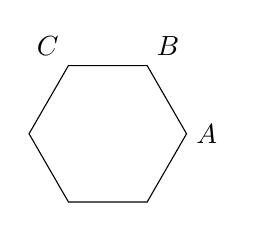
\begin{tikzpicture}
    \draw (0:1) -- (60:1) -- (120:1) -- (180:1) -- (240:1) -- (300:1) -- cycle;
    \node[anchor=west] at (0:1) {$A$};
    \node[anchor=south west] at (60:1) {$B$};
    \node[anchor=south east] at (120:1) {$C$};
\end{tikzpicture}
}

\element{serway-mc}{
\begin{question}{serway-ch04-q63}
    Newton approximated motion in a circle as a series of linear motions,
        as in the polygon below.
    \begin{center}
        \serwayChFourQSixtyThree
    \end{center}
    If we assume the particle moves at constant speed $v_A$ from $A$ to $B$,
        and at constant speed $v_B$ from $B$ to $C$,
        the direction of the change in velocity, $\Delta \vec{\mathbf{v}}$,
        at point $B$, is shown by the arrow in:
    \begin{multicols}{2}
    \begin{choices}
        \AMCboxDimensions{down=-0.8cm}
        \wrongchoice{
            \begin{tikzpicture}
                \draw[dashed,draw=white!50!black] (0,-1) rectangle (-2.0,+1.0);
                \draw[fill] (0,0) circle (1.5pt);
                \draw[thick,->] (0,0) -- (180:2.0cm);
            \end{tikzpicture}
        }
        \wrongchoice{
            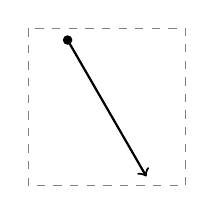
\begin{tikzpicture}
                \draw[dashed,draw=white!50!black] (-0.5,+0.15) rectangle (+1.5,-1.85);
                \draw[fill] (0,0) circle (1.5pt);
                \draw[thick,->] (0,0) -- (-60:2.0cm);
            \end{tikzpicture}
        }
        %% NOTE: ans is C
        \correctchoice{
            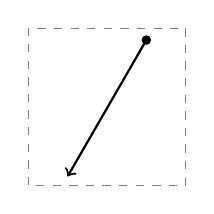
\begin{tikzpicture}
                \draw[dashed,draw=white!50!black] (+0.5,+0.15) rectangle (-1.5,-1.85);
                \draw[fill] (0,0) circle (1.5pt);
                \draw[thick,->] (0,0) -- (240:2.0cm);
            \end{tikzpicture}
        }
        \wrongchoice{
            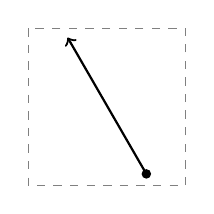
\begin{tikzpicture}
                \draw[dashed,draw=white!50!black] (-1.5,+1.85) rectangle (+0.5,-0.15);
                \draw[fill] (0,0) circle (1.5pt);
                \draw[thick,->] (0,0) -- (120:2.0cm);
            \end{tikzpicture}
        }
        \wrongchoice{
            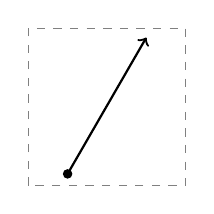
\begin{tikzpicture}
                \draw[dashed,draw=white!50!black] (-0.5,-0.15) rectangle (+1.5,+1.85);
                \draw[fill] (0,0) circle (1.5pt);
                \draw[thick,->] (0,0) -- (+60:2.0cm);
            \end{tikzpicture}
        }
        %% NOTE: symmetry
        \wrongchoice{
            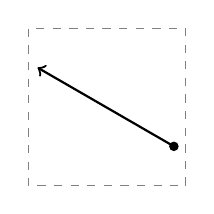
\begin{tikzpicture}
                \draw[dashed,draw=white!50!black] (+0.15,-0.5) rectangle (-1.85,+1.50);
                \draw[fill] (0,0) circle (1.5pt);
                \draw[thick,->] (0,0) -- (+150:2.0cm);
            \end{tikzpicture}
        }
    \end{choices}
    \end{multicols}
\end{question}
}

\element{serway-mc}{
\begin{question}{serway-ch04-q64}
    Newton approximated motion in a circle as a series of linear motions,
        as in the polygon below.
    \begin{center}
        \serwayChFourQSixtyThree
    \end{center}
    If we assume the particle moves at constant speed $v_A$ from $A$ to $B$,
        and at constant speed $v_B$ from $B$ to $C$,
        the direction of the acceleration, $\vec{\mathbf{a}}$, at point $B$,
        is shown by the arrow in:
    \begin{multicols}{2}
    \begin{choices}
        \AMCboxDimensions{down=-0.8cm}
        \wrongchoice{
            \begin{tikzpicture}
                \draw[dashed,draw=white!50!black] (0,-1) rectangle (-2.0,+1.0);
                \draw[fill] (0,0) circle (1.5pt);
                \draw[thick,->] (0,0) -- (180:2.0cm);
            \end{tikzpicture}
        }
        \wrongchoice{
            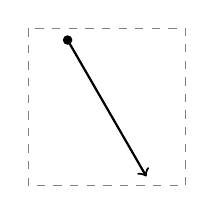
\begin{tikzpicture}
                \draw[dashed,draw=white!50!black] (-0.5,+0.15) rectangle (+1.5,-1.85);
                \draw[fill] (0,0) circle (1.5pt);
                \draw[thick,->] (0,0) -- (-60:2.0cm);
            \end{tikzpicture}
        }
        %% NOTE: ans is C
        \correctchoice{
            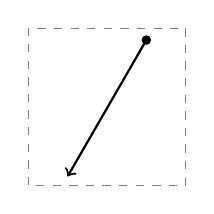
\begin{tikzpicture}
                \draw[dashed,draw=white!50!black] (+0.5,+0.15) rectangle (-1.5,-1.85);
                \draw[fill] (0,0) circle (1.5pt);
                \draw[thick,->] (0,0) -- (240:2.0cm);
            \end{tikzpicture}
        }
        \wrongchoice{
            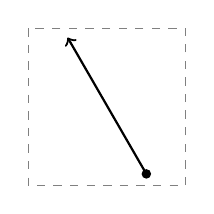
\begin{tikzpicture}
                \draw[dashed,draw=white!50!black] (-1.5,+1.85) rectangle (+0.5,-0.15);
                \draw[fill] (0,0) circle (1.5pt);
                \draw[thick,->] (0,0) -- (120:2.0cm);
            \end{tikzpicture}
        }
        \wrongchoice{
            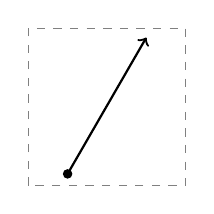
\begin{tikzpicture}
                \draw[dashed,draw=white!50!black] (-0.5,-0.15) rectangle (+1.5,+1.85);
                \draw[fill] (0,0) circle (1.5pt);
                \draw[thick,->] (0,0) -- (+60:2.0cm);
            \end{tikzpicture}
        }
        %% NOTE: symmetry
        \wrongchoice{
            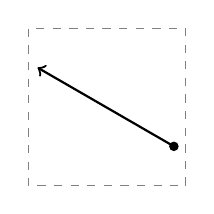
\begin{tikzpicture}
                \draw[dashed,draw=white!50!black] (+0.15,-0.5) rectangle (-1.85,+1.50);
                \draw[fill] (0,0) circle (1.5pt);
                \draw[thick,->] (0,0) -- (+150:2.0cm);
            \end{tikzpicture}
        }
    \end{choices}
    \end{multicols}
\end{question}
}

\element{serway-mc}{
\begin{question}{serway-ch04-q65}
    While the gondola is rising at a speed of \SI{2.0}{\meter\per\second},
        a passenger in a balloon-supported gondola throws a small ball down at a speed of \SI{5.0}{\meter\per\second} relative to his body.
    A person who measures the ball’s velocity at the instant of release will find that the ball’s velocity relative to the ground at that instant is:
    \begin{multicols}{2}
    \begin{choices}
        \wrongchoice{\SI{2.0}{\meter\per\second}, up.}
      \correctchoice{\SI{3.0}{\meter\per\second}, down.}
        \wrongchoice{\SI{3.0}{\meter\per\second}, up.}
        \wrongchoice{\SI{5.0}{\meter\per\second}, down.}
        \wrongchoice{\SI{12.8}{\meter\per\second}, down.}
    \end{choices}
    \end{multicols}
\end{question}
}

\element{serway-mc}{
\begin{question}{serway-ch04-q66}
    While the gondola is rising at a speed of \SI{5.0}{\meter\per\second},
        a passenger in a balloon-supported gondola throws a small ball up at a speed of \SI{2.0}{\meter\per\second} relative to his body.
    A person who measures the ball’s velocity at the instant of release will find that the ball’s velocity relative to the ground at that instant is
    \begin{multicols}{2}
    \begin{choices}
        \wrongchoice{\SI{2.0}{\meter\per\second}, up.}
        \wrongchoice{\SI{2.8}{\meter\per\second}, down.}
        \wrongchoice{\SI{3.0}{\meter\per\second}, up.}
        \wrongchoice{\SI{5.0}{\meter\per\second}, up.}
      \correctchoice{\SI{7.0}{\meter\per\second}, up.}
    \end{choices}
    \end{multicols}
\end{question}
}


\endinput


